%!TEX root = ../thesis.tex

\section{パスの記述と計画における一般的な考慮事項 }
マニピュレータの動きはツールフレーム{T}がステーションフレーム{S}に対してどのように動くか考える.基本的な問題はマニピュレータを初期位置から最終位置まで移動させることである.つまり,ツールフレーム{T}を現在の値から望ましい最終値まで移動させたい.一般的に,この動きにはツールがステーションに対して姿勢と位置の両方が変化することが含まれる. \\

動きを詳細に指定するためには,望ましい経由点(初期位置と最終位置の間の中間点)を指定することがある.これらの経由点は,ツールがステーションに対して位置と姿勢を指定するフレームであり,初期点と最終点と共にパスポイントと呼ばれる.スムーズな動きを実現するためには,関節空間での連続性が必要であり,時間的属性も指定される場合がある.ガタガタした動きは機構の摩耗を増加させ,振動を引き起こすため,経由点間の経路には制約が必要である. \\

\section{関節空間スキーム}
ここでは,パスの生成方法を考えるが,パスの形状(空間及び時間)は関節角度の関数として記述される.通常,各パスポイントはツールフレーム{T}がステーションフレーム{S}に対して望ましい位置と姿勢で指定され,逆運動学を使用して関節角度が計算される.各関節には関係なく,滑らかな関数が見つかり,経由点での望ましい位置と姿勢が実現される.関節空間スキームは通常計算が容易であり,特異点の問題が少ないことが特徴である.  

\subsection{直方体多項式}
ツールを初期位置から目標位置に一定の時間で移動させる問題を考える.各関節には,$t_0$での値が関節の初期位置であり,$t_f$での値がその関節の望ましい目標位置である関数が必要である.\figref{Fig:fig1}に示されているように,関節の値を補間するために使用できる滑らかな関数θ(t)は多くある.スムーズな動きを行うためには,θ(t)に対して少なくとも4つの制約がある.関数に対する2つの制約は初期値と最終値の選択から来る. 

$$ θ(0)=θ_0$$
$$ θ(t_f)=θ_f \eqno(1)$$

\begin{figure}[h]
     \centering
     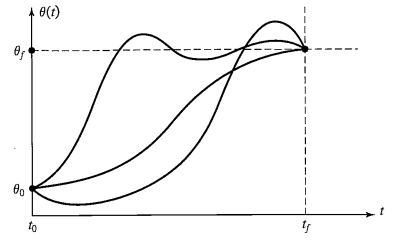
\includegraphics[keepaspectratio, scale=0.6]{images/fig1.png}
     \caption{}
     \label{Fig:fig1}
     \end{figure}

さらに2つの制約は,この関数が速度で連続であることであり,これは初期速度と最終速度がゼロであることを意味する.

$$\dot{θ}(0) = 0$$
$$\dot{θ}(t_f) = 0 \eqno(2)$$

これら4つの制約は,少なくとも3時の多項式で満たすことができる.(3時多項式は4つの係数を持つため,式(1)と(2)で与えられる4つの制約を満たすようにできる.)これらの制約によって特定の3次多項式が一意に決定される.3次多項式は次のようになる.

$$θ(t) = a_0 + a_1t + a_2t^2 + a_3t^3 \eqno(3)$$

従ってこのパスに沿った関節の速度と加速度は明確に決まる

$$\dot{θ}(t) = a_1 + 2a_2t + 3a_3t^2$$
$$\ddot{θ}(t) = 2a_2 + 6a_3t \eqno(4)$$

式(3)と(4)を4つの制約と組み合わせることで,4つの未知数に対する4つの方程式が得られる. 

$$θ_0 = a_0$$
$$θ_f = a_0 + a_1t_f + a_2t_f^2 + a_3t_f^3$$
$$0 = a_1 \eqno(5)$$
$$0 = a_1 + 2a_2t_f + 3a_3t_f^2$$

これらの方程式を解くと以下の結果が得られる. 

$$a_0 = θ_0$$
$$a_1 = 0$$
$$a_2 = \frac{3}{t_f^2}(θ_f-θ_0) \eqno(6)$$

式(6)を使用することで,任意の初期関節角度位置と望ましい最終位置を接続するための3次多項式を計算できる.この解は,関節が速度ゼロで始まり,速度ゼロで終わる場合のケースに対してのものである.